\label{sec:sokar-scenesets}

Abstrakcyjna klasa \sokarclass{DicomSceneSet} implementuje wektor scen za pomocą klasy \qtclass{QVector}.
Jest to obiekt, który przechowuje sceny i tworzy sekwencje scen, która jest rzeczywistym ułożeniem ramek obrazów.
Są dwie implementacje kolekcji scen: kolekcja plików i kolekcja ramek z jednego pliku.
Diagram klas UML znajduje się na rysunku \ref{uml:sokar-scene-sets}.

\begin{figure}[!htbp]
    \centering
    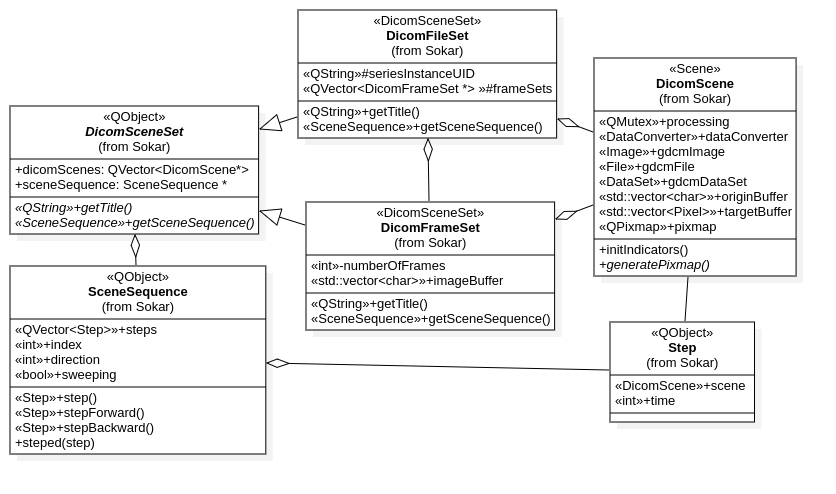
\includegraphics[width=\textwidth]{img/uml/sokar-scene-sets.png}
    \caption{Diagram klas UML dziedziczenia klasy \sokarclass{DicomSceneSet}.}
    \label{uml:sokar-scene-sets}
\end{figure}

\subsubsection{Sekwencja scen}
\label{sec:sokar-scenesequence}

\par
Sekwencja scen implementuje strukturę danych informującą o przejściach pomiędzy scenami poprzez klasę \sokarclass{SceneSequence}.
Sekwencja to wektor zawierający kroki z dodatkowymi informacjami o stanie sekwencji:
\begin{itemize}
    \item indeks, w którym obecnie znajduje się sekwencja,
    \item kierunek sekwencji --- sekwencja może iść w stronę początku lub końca,
    \item rodzaj przemiatania --- wartość logiczna informująca w jaki sposób ma zachować się, gdy sekwencja dojdzie do końca, lub początku.
\end{itemize}
Po dojściu do końca sekwencja skoczy do pierwszego elementu lub może zmienić kierunek i zacząć iść do tyłu.

\par
Kroki implementowane przez klasę \sokarclass{Step} zawierają następujące informacje: wskaźnik do sceny oraz czas trwania sceny.

\par
Sekwencja ma wbudowane funkcje zapewniające przesuwanie się po indeksie na wektorze:
\begin{itemize}
    \item \sokarfunction{SceneSequence}{stepForward} --- krok do przodu --- zwiększa indeks tym samym wykonując krok w stronę końca sekwencji,
    \item \sokarfunction{SceneSequence}{stepBackward} --- krok do tyłu --- zmniejsza indeks tym samym wykonując krok w stronę początku sekwencji,
    \item \sokarfunction{SceneSequence}{step} --- wykonuje krok w tył lub przód w zależności od kierunku sekwencji.
\end{itemize}
Wszystkie powyższe funkcje są zarazem slotami dla sygnałów oraz emitują sygnał \sokarfunction{SceneSequence}{steped}.

\subsubsection{Kolekcja ramek \DICOM}
\label{sec:sokar-dicomframeset}

\par
Zbiory ramek są implementowane przez \sokarclass{DicomFrameSet} i są tworzone z jednego wczytanego pliku \DICOM.
Klasa tworzy obiekt konwertera i pobiera liczbę ramek w obrazie.
Tworzy jeden buffor na wszystkie ramki obrazów, a następnie dzieli go na ilość ramek.
Biblioteka GDCM nie daje dostępu do oryginalnego bufora, dlatego wymagany jest bufor pośredni.
Następnie jest tworzonych tyle obiektów scen ile jest ramek.
\par
Kolejność sekwencji scen jest taka sama jak kolejność ramek.
Natomiast czas wyświetlania ramki może być zapisany w różnych znacznikach.
To, w którym znaczniku został zapisany, informuje element o znaczniku \dicomtag{Frame Increment Pointer}{0028}{0009}.
Zawiera on wskaźnik do elementu o zadanym znaczniku.
\par
Została zaimplementowana obsługa poniższych znaczników:
\begin{itemize}
    \item \dicomtag{Frame Time}{0018}{1063} --- element z tym znacznikiem zawiera czas trwania jednej ramki w milisekundach.
          Każdemu krokowi jest przypisywana ta wartość trwania.

    \item \dicomtag{Frame Time Vector}{0018}{1065} --- zawiera tablice z przyrostami czasu w milisekundach między n-tą ramką a poprzednią klatką.
          Pierwsza ramka ma zawsze przyrost czasu równy 0.

    \item \dicomtag{Cine Rate}{0018}{0040} --- zawiera ilość klatek wyświetlanych na sekundę.
          Każdemu krokowi jest przypisywana wartość do niej odwrotna.
\end{itemize}
W przypadku braku znacznika lub gdy zostaje wskazany znacznik nieznany, czas trwania ramki wynosi $83.3$ milisekundy, co odpowiada 12 klatkom na sekundę.


\subsubsection{Kolekcja plików \DICOM}
\label{sec:sokar-dicomfileset}
\par
Zbiory plików są implementowane przez \sokarclass{DicomFileSet} i służą do przechowywania wielu wczytanych plików \DICOM.
Na początku pliki są sortowane na podstawie liczby zawartej w elemencie o znaczniku \dicomtag{Instance Number}{0020}{0013}.
Dla każdego pliku jest tworzony obiekt \sokarclass{DicomFrameSet}.
\par
Sekwencja jest tworzona poprzez połączenie sekwencji poszczególnych obrazów.

\subsubsection{Segregowanie obrazów}
\label{sec:sokar-dicomfileset-create}
\par
W przypadku kiedy mamy do czynienia z wieloma plikami, należy jest rozdzielić na serie i uporządkować w odpowiedniej kolejności.
Unikalny identyfikator serii jest zawarty w elemencie danych o znaczniku \dicomtag{Series Instance UID}{0020}{000E}.
Kolejności obrazów w serii to liczba zawarta w elemencie danych o znaczniku \dicomtag{Instance Number}{0020}{0013}.
\par
Segregacja odbywa się za pomocą funkcji \sokarfunction{DicomFileSet}{create}.
Do funkcji jest przesyłany wektor z wczytanymi plikami \DICOM, następnie dzieli ona pliki na zbiory zawierające zdjęcia tej samej serii, tworzy obiekty zbiorów plików \DICOM.
Ostatecznie zwraca ona wektor z gotowymi obiektami zbiorów plików \DICOM.
Sortowanie plików \DICOM według ich kolejności odbywa się za pomocą funkcji \stdclass{sort}{algorithm/sort} wewnątrz konstruktora klasy \sokarclass{DicomFileSet}, który nie jest publiczny.